

%..--..--..--..--..--..--..--..--..--..--..--..--..--..--..--..--..--..--..--..--..--..--..--..--..--..--..--..--..--..--..--..
%\subsubsection{$\pi$-{\sc Pews}  meta-model}\label{sec:pewsmetamodel}
%..--..--..--..--..--..--..--..--..--..--..--..--..--..--..--..--..--..--..--..--..--..--..--..--..--..--..--..--..--..--..--..

\pisodm  proposes intra-level transformation rules between $\pi$-use case to $\pi$-service process models, $\pi$-service process to $\pi$-service composition  models, as well as inter-level transformation rules between $\pi$-service composition to $\pi$-PEWS models. 
These rules are used to build a semi-automatic tool.
The transformations from CIM to PIM level models is not automatized, due to the informal nature of CIM level representations.
 
% _ . _ . _ . _ . _ . _ . _ . _ . _ . _ . _ . _ . _ . _ . _ . _ . _ . _ .
\subsection{From $\pi$-UseCase to the $\pi$-ServiceProcess}
% _ . _ . _ . _ . _ . _ . _ . _ . _ . _ . _ . _ . _ . _ . _ . _ . _ . _ .

The refinement of a (composite) $\pi$-Use Case model into a $\pi$-Service Process model is driven by the principle of expressing a set of $\pi$-use cases (i.e., use cases with constraints)   in terms of  a business process.
The resulting model consists of actions related by a control flow and contracts specifying NFPs. 

As defined by the $\pi$-ServiceProcess  meta-model (Figure~\ref{fig:CIM:serviceprocessmetamodel}) an {\sc Activity Service} consists of a composition of  entities of type {\sc Action}. 
Thus, every {\sf $\pi$-use case} is transformed into an {\sf Action} of the target $\pi$-Service Process model.  
Every {\sf Extend} relationship identified in a $\pi$-Use Case model is transformed into a  {\sf Fork node}\footnote{Notice that Fork nodes are used both to represent alternative and parallel execution. {\color{red} \sc Placido, please check this!}}.
If the {\sf Extend} relationship concerns just one {\sf use case}, it is transformed into an {\sf Action} inside one flow of the fork node. 
Otherwise, several  {\sf use cases} are transformed into different {\sf Actions} that belong to different flows departing from the fork node.   

%\begin{figure}
%\centering{
%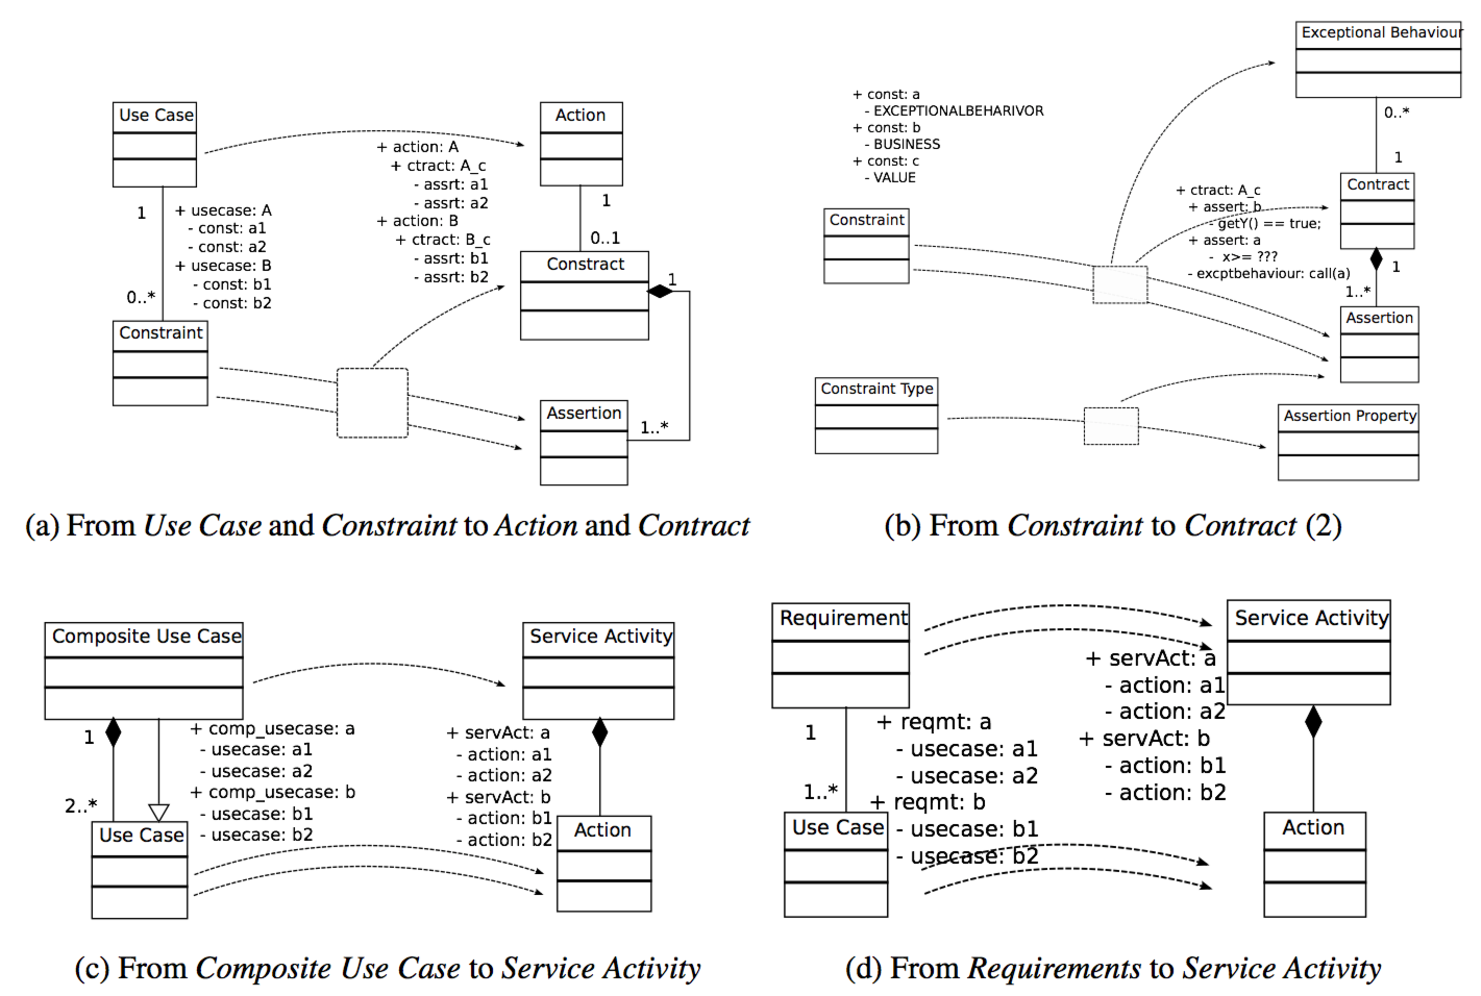
\includegraphics[width=0.96\textwidth]{figs/35}}
%\caption{ $\pi$-UseCase to $\pi$-ServiceProcess transformation rules}
%\label{fig:transformationsUseCase-ServiceProcessRules}
%\end{figure}

A {\sf Constraint} associated to a {\sf Use Case}  is transformed into an  {\sf Assertion}.  
The set of resulting assertions  are grouped into a {\sf Contract}.
Constraints are transformed according to their type:
{\sc Business} constraints and {\sc Value} constraints with the {\sf  isExceptionalBehaviour} attribute set to false are transformed into {\sf Assertion}s;
{\sc Value } constraints with the {\sf  isExceptionalBehaviour} attribute set to true are transformed into {\sf Exceptional behaviour}s.

In order to transform constraints of type {\sf Value Constraint}, the designer must specify thresholds to be associated to the assertions of a contract.
By default, value constraints are transformed into pre-conditions and business constraints are transformed into post-conditions. 
  
%A {\sf Requirement} and a {\sf Composite use case} in a  $\pi$-UseCase model are transformed respectively into a {\sf Service activity} and an {\sf Action} (see figures  \ref{fig:transformationsUseCase-ServiceProcessRules}-c  and d). 
%
%
%\begin{figure}
%\centering{
%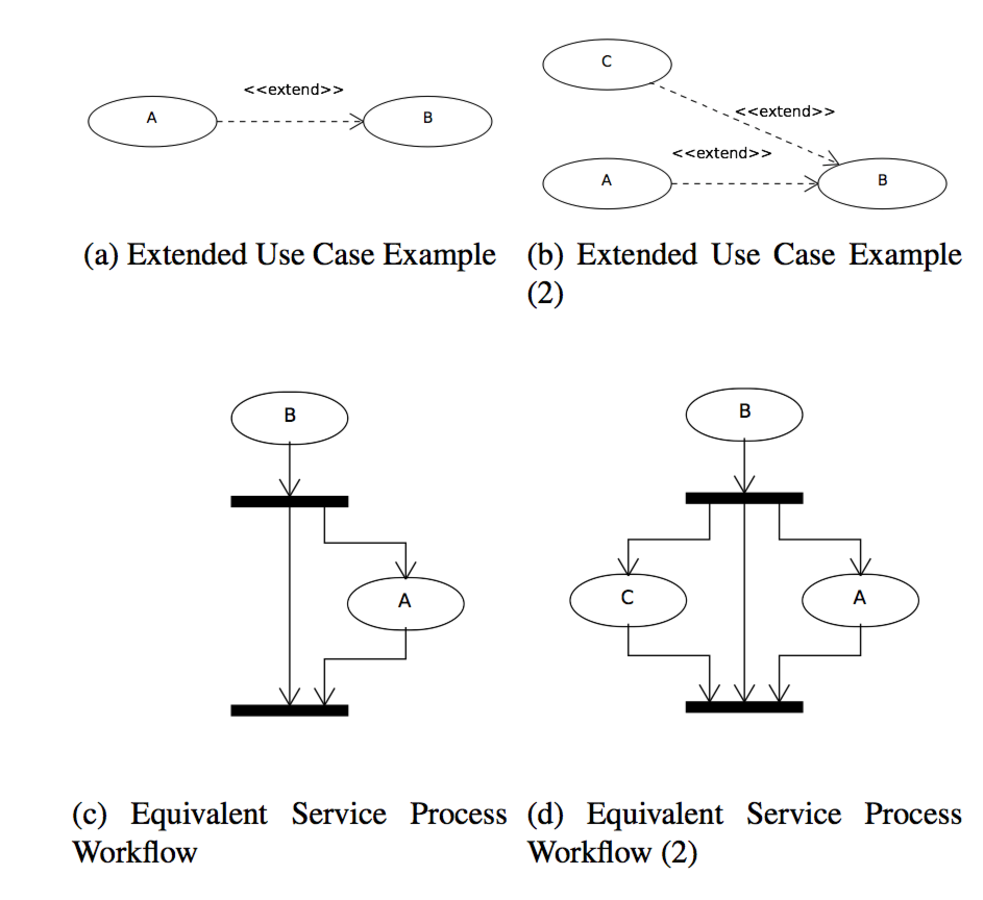
\includegraphics[width=0.80\textwidth]{figs/37}}
%\caption{ Extended Transformation Examples}
%\label{fig:transformaton-examples}
%\end{figure}

%The transformations for {\sc Extend} and {\sc Include} dependencies  are not as simple as the previous transformations (figures \ref{fig:transformaton-examples}-a). 

The relationships of type  {\sc Extend} and {\sc Include}  determine the way the business process is expressed as a workflow.  
The generated workflow is composed by {\sf Fork} and {\sf Join} nodes,  {\sc Control flow} constructors, as well as entities of type {\sc Action}.

%\begin{figure}
%\centering{
%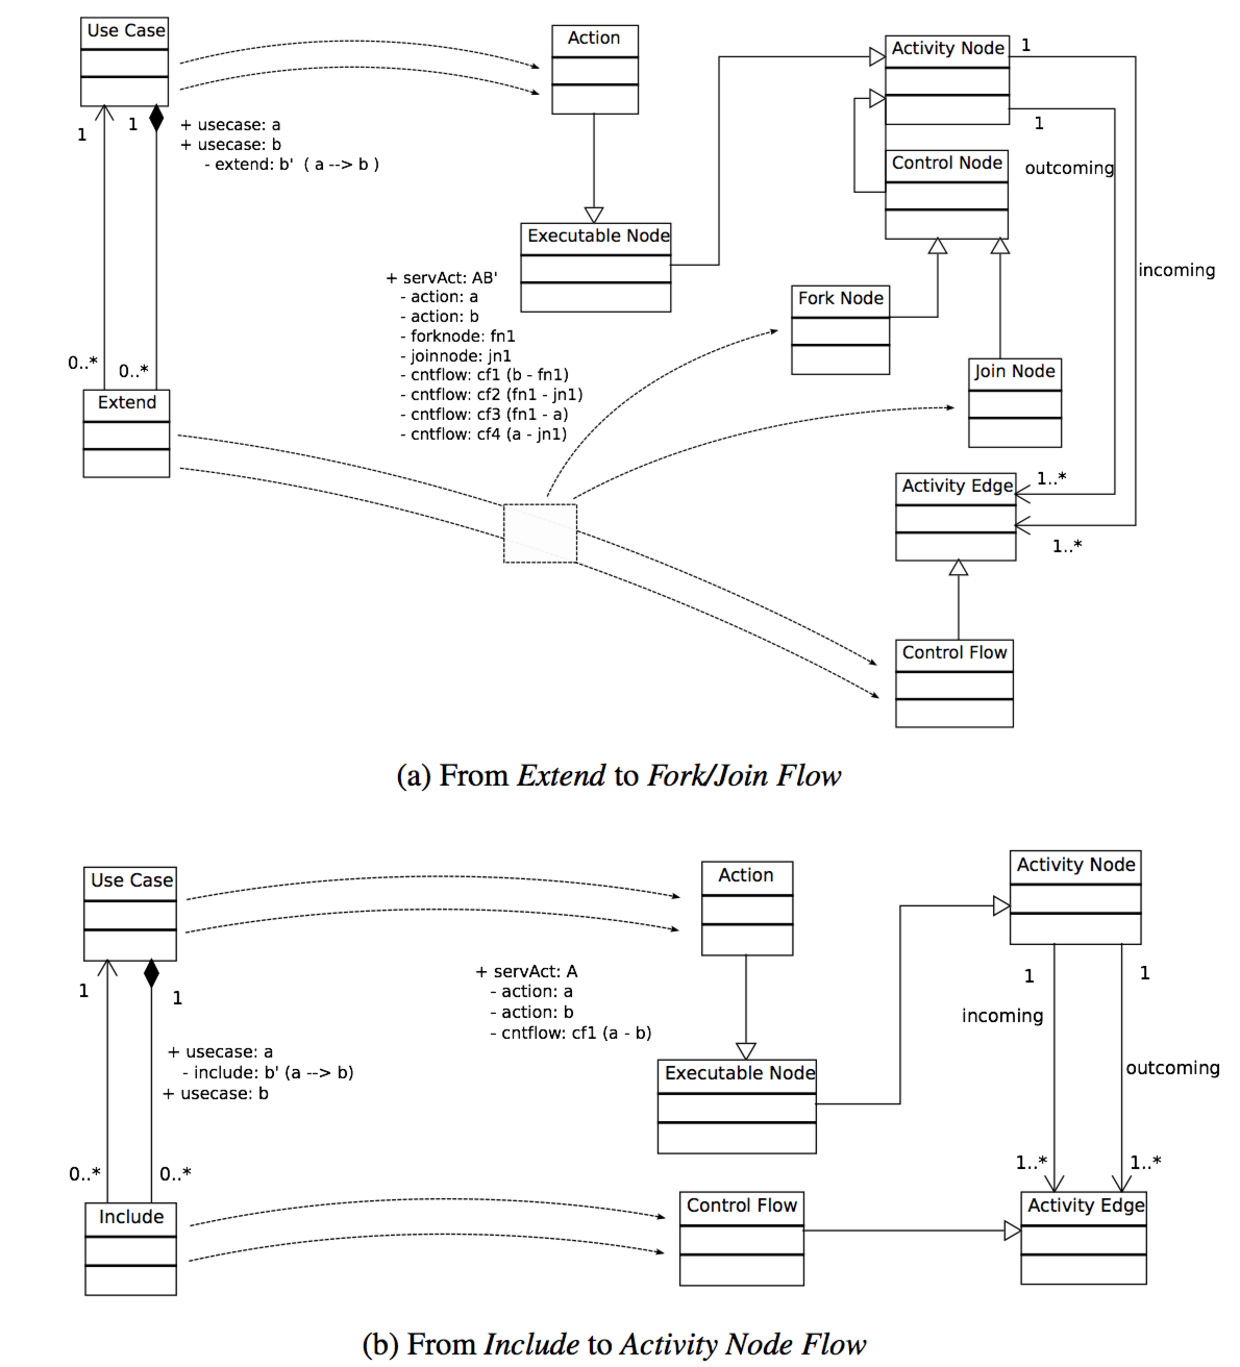
\includegraphics[width=0.96\textwidth]{figs/36}}
%\caption{ $\pi$-UseCase to $\pi$-ServiceProcess Model Transformation Rules (2)}
%\label{fig:transformationsUseCase-ServiceProcessRules}
%\end{figure}

{\sf Include} use case entities are transformed into an {\sf Action} sequence.
A {\sc Use case} element is transformed into an {\sf Action}. 
A set of $n$ {\sc Use cases} is transformed into an  $n-1$ {\sf Object flow} elements. 

The details of these transformations are not included here (due to space restrictions).
They can be found in~\cite{SouzaNeto:2012}.

\begin{example}[To Publish Music \textit{(cont)}]\label{ex:toPublicMusicT1}
The rules presented above have been applied to the model in Figure~\ref{fig:piUseCaseModel}, in order to obtain the $\pi$-Service Process model for our running example (Figure~\ref{fig:CIM:serviceprocess}).

The ``listen music'' use case is transformed into a Service Action. 
This Action  represents a Spotify service function that can be invoked to play the music. 
For the ``publish music'' use case,  constraints are transformed into a set of assertions that are grouped into a Contract ({\sf ``publishMusicContract''}) associated to the Action {\sf ``publishMusic''}. 
The ``download music'' use case  includes the payment process to buy the music. 
Thus, these use cases  are transformed into {\sf Actions}, and a {\sf Service Activity} that aggregates these {\sf Actions}.   
This \textsf{Service Activity} is transformed into a sequence flow on the $\pi$-service process model.
%(as shown in figure \ref{fig:transformation-example-include}). 
The same rule is applied for the ``publish music'' use case, which has two extended use cases, to publish on Twitter and Facebook.
 \end{example}

%\begin{figure}
%\centering{
%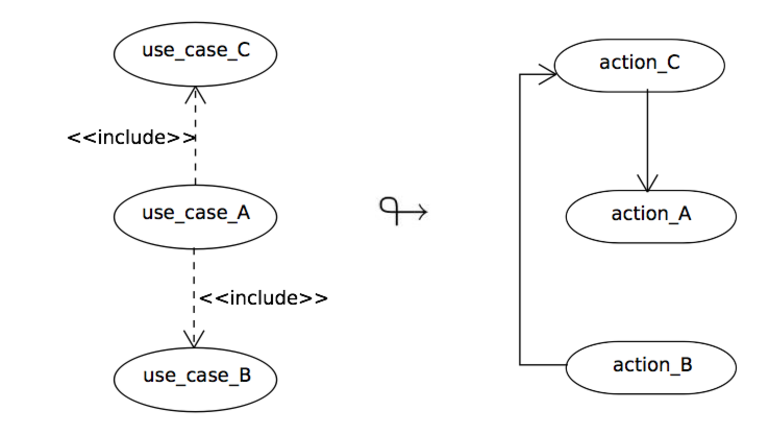
\includegraphics[width=0.76\textwidth]{figs/38}}
%\caption{ Include Transformation Example}
%\label{fig:transformation-example-include}
%\end{figure}


PARAMOS AQUIIIIIIIIIIIIIIIIIIIIIIIIIIIIIIIIIIIIIIIIIIIIIIIIIIIIIII

% _ . _ . _ . _ . _ . _ . _ . _ . _ . _ . _ . _ . _ . _ . _ . _ . _ . _ .
\subsection{From $\pi$-ServiceProcess to $\pi$-ServiceComposition}
% _ . _ . _ . _ . _ . _ . _ . _ . _ . _ . _ . _ . _ . _ . _ . _ . _ . _ .
%The {\em A-policies} defined for the elements of the $\pi$-SCM are transformed into {\sc A-Policy} classes, named according to the names expressed in the source model. The transformation of the rules expressed in the $\pi$-SCM is guided by the event types associated to these rules.   The variables associated to an {\em A-policy} expressed in the $\pi$-SCM as {\sc\em $<$Variable:name, Variable:type$>$} are transformed into elements of type {\sc Variable} with attributes {\sc name} and {\sc type} directly specified from the elements {\sc\em  Variable:name} and {\sc\em Variable:type} of the $\pi$-SCM model.

%As shown in Figure \ref{fig:transformations}, for an event of type {\sc\em Pre} the corresponding transformed rule is of type {\sc Precondition}; for an event of type {\sc\em Post} the corresponding transformed rule is of type {\sc Postcondition}; finally, for an event of type {\sc\em TimeRestriction} the corresponding transformed rule is of type {\sc Time}. 
%The condition expression of a rule in the $\pi$-SCM ({\sc\em Rule:condition}) is transformed into a class {\sc\em Condition:expression} where the attributes of the expression are transformed into elements of type {\sc Attribute}.

%The attribute event of a rule  ({\sc\em Rule:event}) in the $\pi$-SCM is transformed into an {\sc Event Type} according to the rule type. 

%As shown in Figure \ref{fig:transformations}, the event type for a rule of type (i) {\sc Precondition} is {\sc ActivityPrepared}; (ii) {\sc Postcondition} is {\sc TermActivity}; (iii) {\sc TimeRestriction} is {\sc Temporal}. The {\sc\em Rule:Action} of a rule in the $\pi$-SCM is transformed into an {\sc Action:type}.

%
%Figure \ref{fig:p-scim} shows the  $\pi$-{\sc Pews} model for our example.
%In the scenario "To Publish Music" the {\sf Policies} {\em OAuthPolicy} and {\em HTTPAuthPolicy} of the $\pi$-SCM model are transformed into {\em A-policies} of type {\sf Precondition} of the $\pi$-{\sc Pews} model of the scenario. Thus in both cases the events are of type {\sf ActivityPrepared}. These policies, as stated in the $\pi$-SCM model, are associated to {\sf Activities}. In the corresponding transformation they are associated to {\sf Operation}s {\em PublishFacebook} and {\em PublishTwitter}.
%\begin{figure}[htpb]
%\centering{
%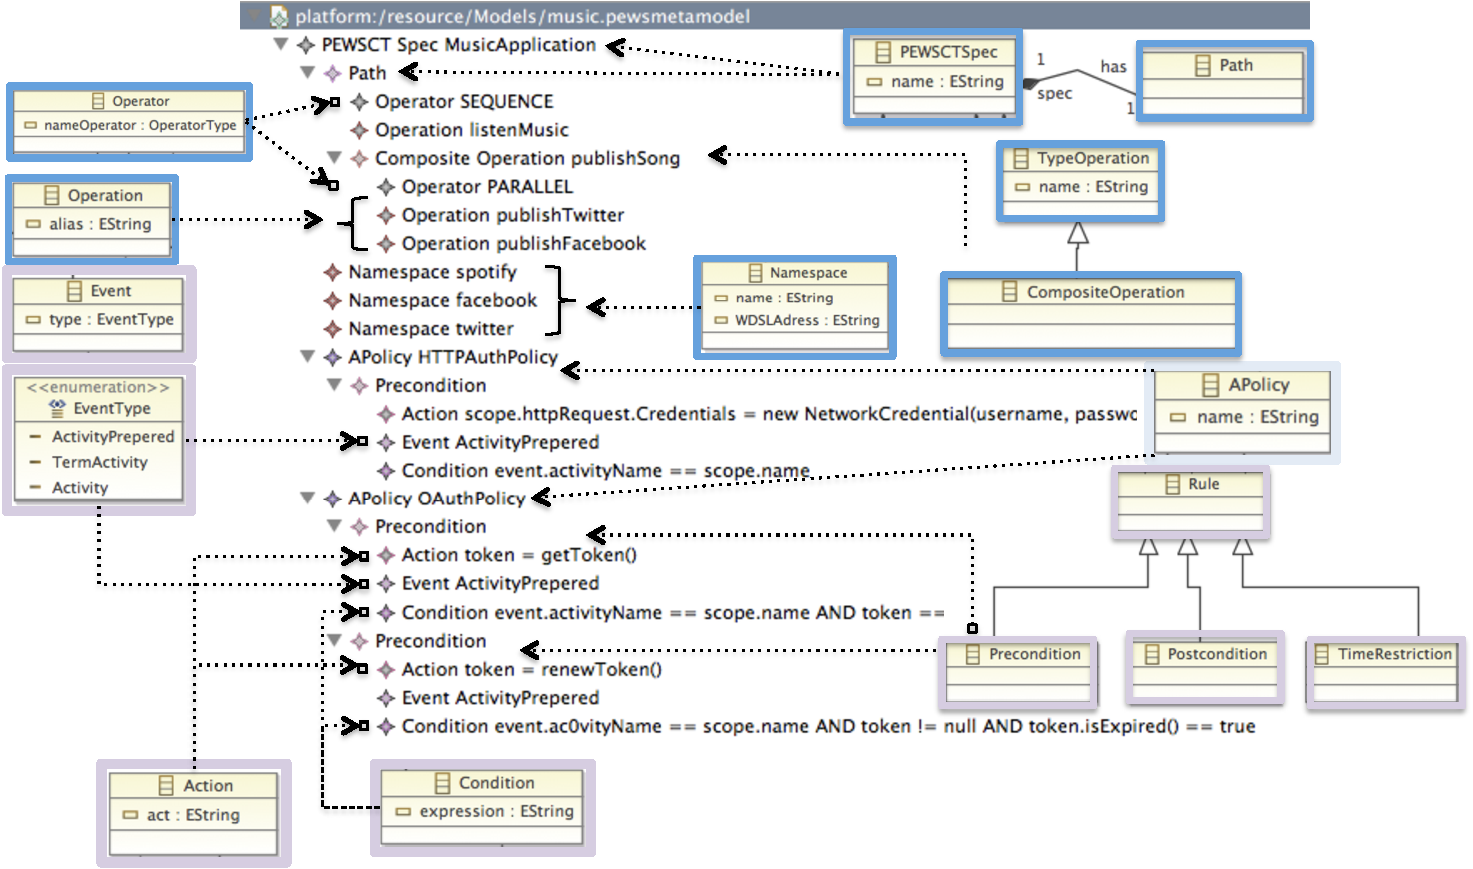
\includegraphics[width=0.78\textwidth]{figs/modeloPEWS}}
%\caption{$\pi$-{\sc Pews} generated model fo the "To Publish Music" application}
%\label{fig:p-scim}
%\end{figure}

%Figure \ref{fig:pewsexpression} shows the correspondence between the model and the statements that implement it, with a schematic representation of the business process.
%\begin{figure}
%\centering{
%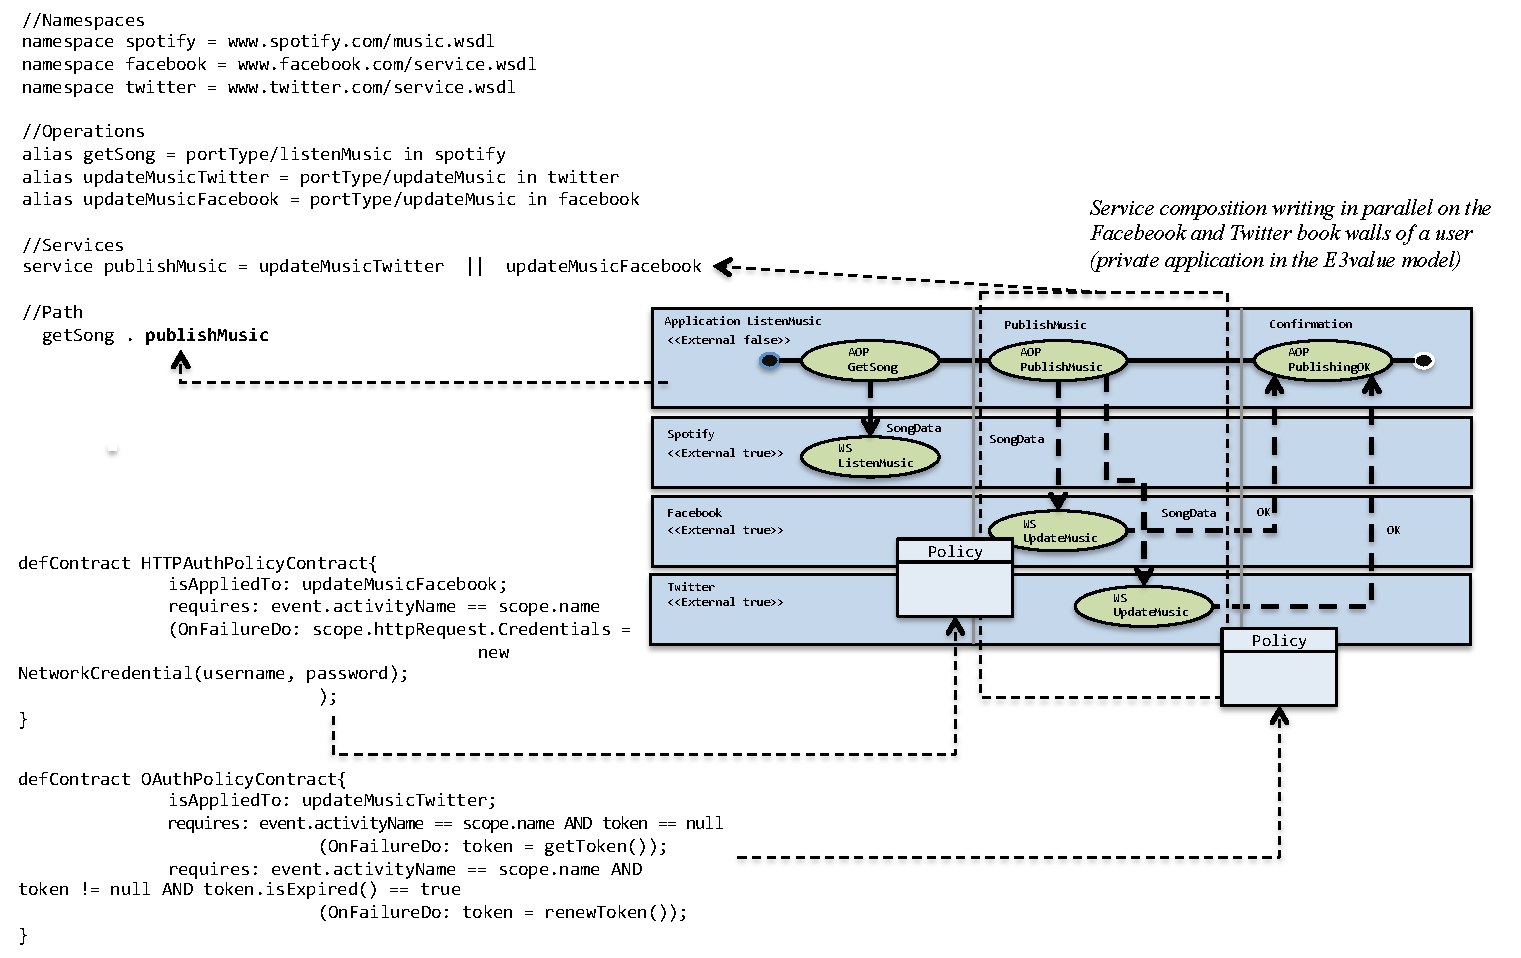
\includegraphics[width=0.85\textwidth]{figs/pews-expression}}
%\caption{Pews program implementing the "To Publish Music" application}
%\label{fig:pewsexpression}
%\end{figure}
%Table \ref{fig:ServiceProcess-ServiceComposition}  shows the transformation rules for transforming a .
As illustrated in Figure \ref{fig:ServiceProcess-ServiceComposition-Rules} the  principle of the transformation  of a  $\pi$-Service process model into a   $\pi$-ServiceComposition model is to group respectively  {\sf Contracts}  and {\sf Actions} into {\sf Policies} and {\sf Service activities}.   

Each {\sf Assertion} of a {\sf Contract} in a $\pi$-service composition model is transformed into a {\sf Rule} in a $\pi$-service composition model. The set of {\sf Rules}  concerning the same NFP (e.g., safety, performance, and reliability) is grouped into a {\sf Policy} (see Figure \ref{fig:ServiceProcess-ServiceComposition-Rules}-a). Each {\sf Assertion} of a {\sf Contract} is transformed into a {\sf Rule:Condition} attribute. If the {\sf Assertion} has a value type, the name and the attributes are transformed into a {\sf Variable} in the target model.  The {\sf Assertion: Aproperty} attribute can have different transformations, according to  the following rules:
\begin{itemize}
\item a {\sf Post-Condition} is transformed into a {\sf  Post}. 
\item a {\sf Precondition} is transformed into {\sf Pre}.
\item a {\sf Timerestriction} is transformed into {\sf Time}.
\end{itemize}


\begin{figure}
\centering{
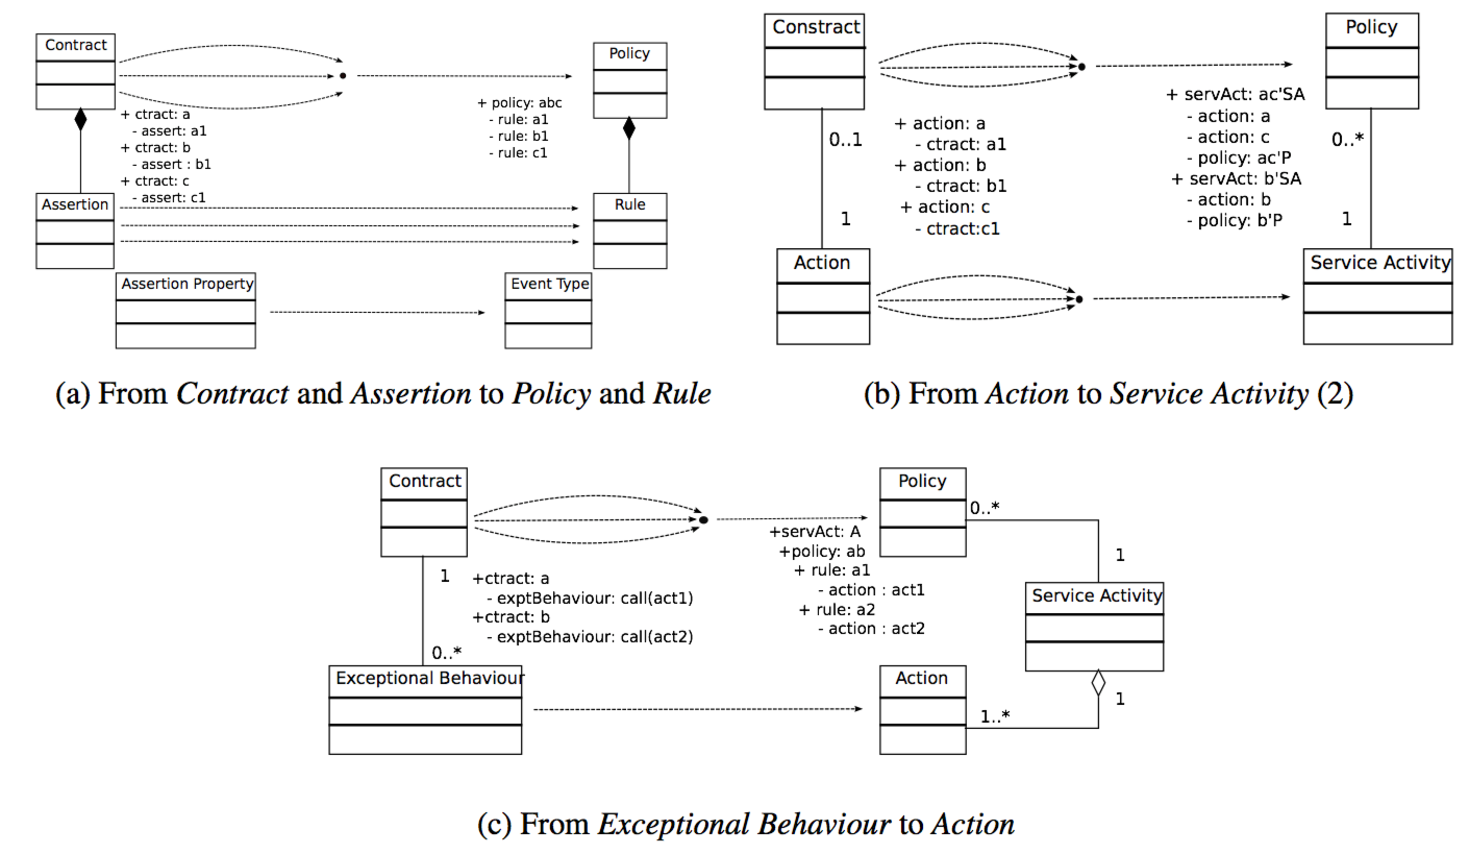
\includegraphics[width=0.96\textwidth]{figs/ExceptionalRules}}
\caption{$\pi$-ServiceProcess to $\pi$-ServiceComposition Model Transformation Rules}
\label{fig:ServiceProcess-ServiceComposition-Rules}
\end{figure}

A {\sf Package}  in the $\pi$-use case model is transformed   into a {\sf Business Collaborator}. 
{\sf Actions}  of a $\pi$-service process model are transformed into an {\sf Action} in a $\pi$-service composition model, and every {\sf Service activity} of a $\pi$-service process model is transformed into a {\sf Service activity} in a $\pi$-service composition model (see Figure \ref{fig:ServiceProcess-ServiceComposition-Rules}-b). An {\sf Exceptional behaviour} entity is transformed into an {\sf Action} in a $\pi$-service composition model (see Figure \ref{fig:ServiceProcess-ServiceComposition-Rules}-c ), and every {\sf Non-functional attribute} associated to an element ({\sf Contract} and {\sf Non-functional requirement}) in a $\pi$-service process model becomes a {\sf Non-functional attribute} associated to the corresponding element {\sf Policy} in a $\pi$-service composition model.
 Finally, {\sf Actions} are grouped by  a  {\sf Business collaborator}.  

%\begin{figure}
%\centering{
%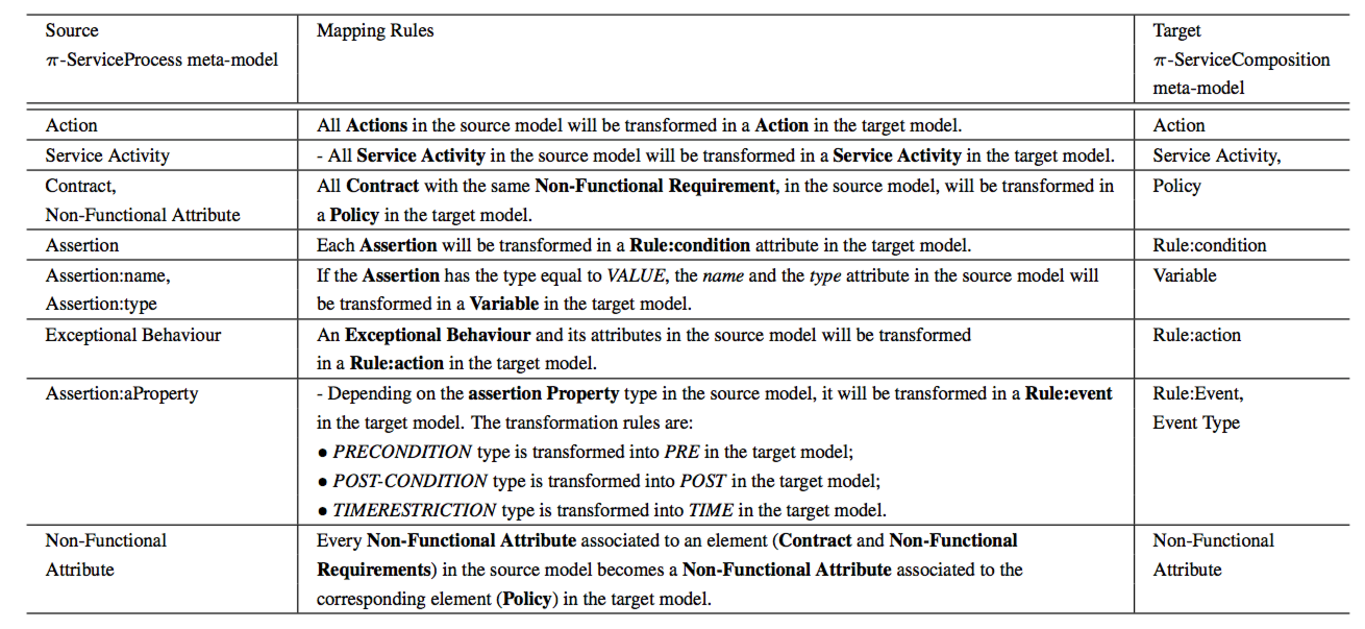
\includegraphics[width=1\textwidth]{figs/ServiceProcess-ServiceComposition}}
%\caption{ Transformation Rules: From $\pi$-ServiceProcess to $\pi$-ServiceComposition}
%\label{fig:ServiceProcess-ServiceComposition}
%\end{figure}






%As the $\pi$-ServiceComposition model refines the $\pi$-ServiceProcess concepts at PIM level, a service previously defined as actions (source model) is refined as composition of those actions (target model) that are necessary to represent a business service, identifying who are the partners involved in the realization ({\sc Business collaborators}). 
%In addition, $\pi$-SOD-M defines a platform specific model based on web services composition. This model is explicitly indicates those actions which are (or will be, if not yet implemented) supported by web services.

\begin{example}[To Publish Music \textit{(cont)}]\label{ex:toPublicMusicT5}
Considering the scenario example, 
%the {\sf Action}s update music {\sc Contract} is transformed is a {\sc Policy} with its {\sc Rules}. All contract {\sc Assertions} are transformed in RULE and its attributes, e.g. the login and password verification. 
the "securityLoginPolicy" consists of a set of {\sf Rules} that were transformed from the {\sf Assertions} in $\pi$-service process model. 
%The {\sc Non- functional requirement} information will be used to the {\sc Policy} generation comes from the initial use case model. Also 
The {\sf Business Collaborator} Facebook and Spotify information come from entity of type {\sc Package}  in the $\pi$-use case model. 
%All {\sc Contracts} of the same {\sc Non- functional requirement} are composed in a {\sc Policy}.
\end{example}

% _ . _ . _ . _ . _ . _ . _ . _ . _ . _ . _ . _ . _ . _ . _ . _ . _ . _ .
\subsection{From $\pi$-ServiceComposition to $\pi$-PEWS}
% _ . _ . _ . _ . _ . _ . _ . _ . _ . _ . _ . _ . _ . _ . _ . _ . _ . _ .

%Table \ref{fig:ServiceComposition-Pews-Rules} 
This section describes the PIM to PSM transformations from a $\pi$-Service composition model to a $\pi$-PEWS program. We propose two groups of rules: those that transform services composition entities of a $\pi$-Service composition model into $\pi$-PEWS model; and those that transform rules grouped by policies into A-policy types.

A named action of the $\pi$-service composition model represented by  {\sf Action} and {\sf Action:name} is transformed to an  {\sf Operation} with a corresponding attribute name {\sf Operation:name}. A  named service activity represented by the elements {\sf ServiceActivity}  and  {\sf ServiceActivity:name} of the $\pi$-service composition model, are  transformed into a named operation of the $\pi$-{Pews} represented by the entities  {\sf CompositeOperation} and {\sf CompositeOperation:name}. When more than one action is called, according to the following  composition patterns expressed using the operators {\sc\em merge, decision, fork and join} in the $\pi$-service composition model the corresponding transformations, according to the PEWS operators presented above:
\begin{itemize}
\item   $op_1 . op_2$ if no {\sc\em ControlNode} is specified
\item ($op_1 \parallel op_2) . op_3$ if control nodes of type {\sc\em fork, join} are combined
 \item ($op_1 + op_2) . op_3$ if control nodes of type {\sc\em decision, merge} are combined
\end{itemize}

%\begin{figure}
%\centering{
%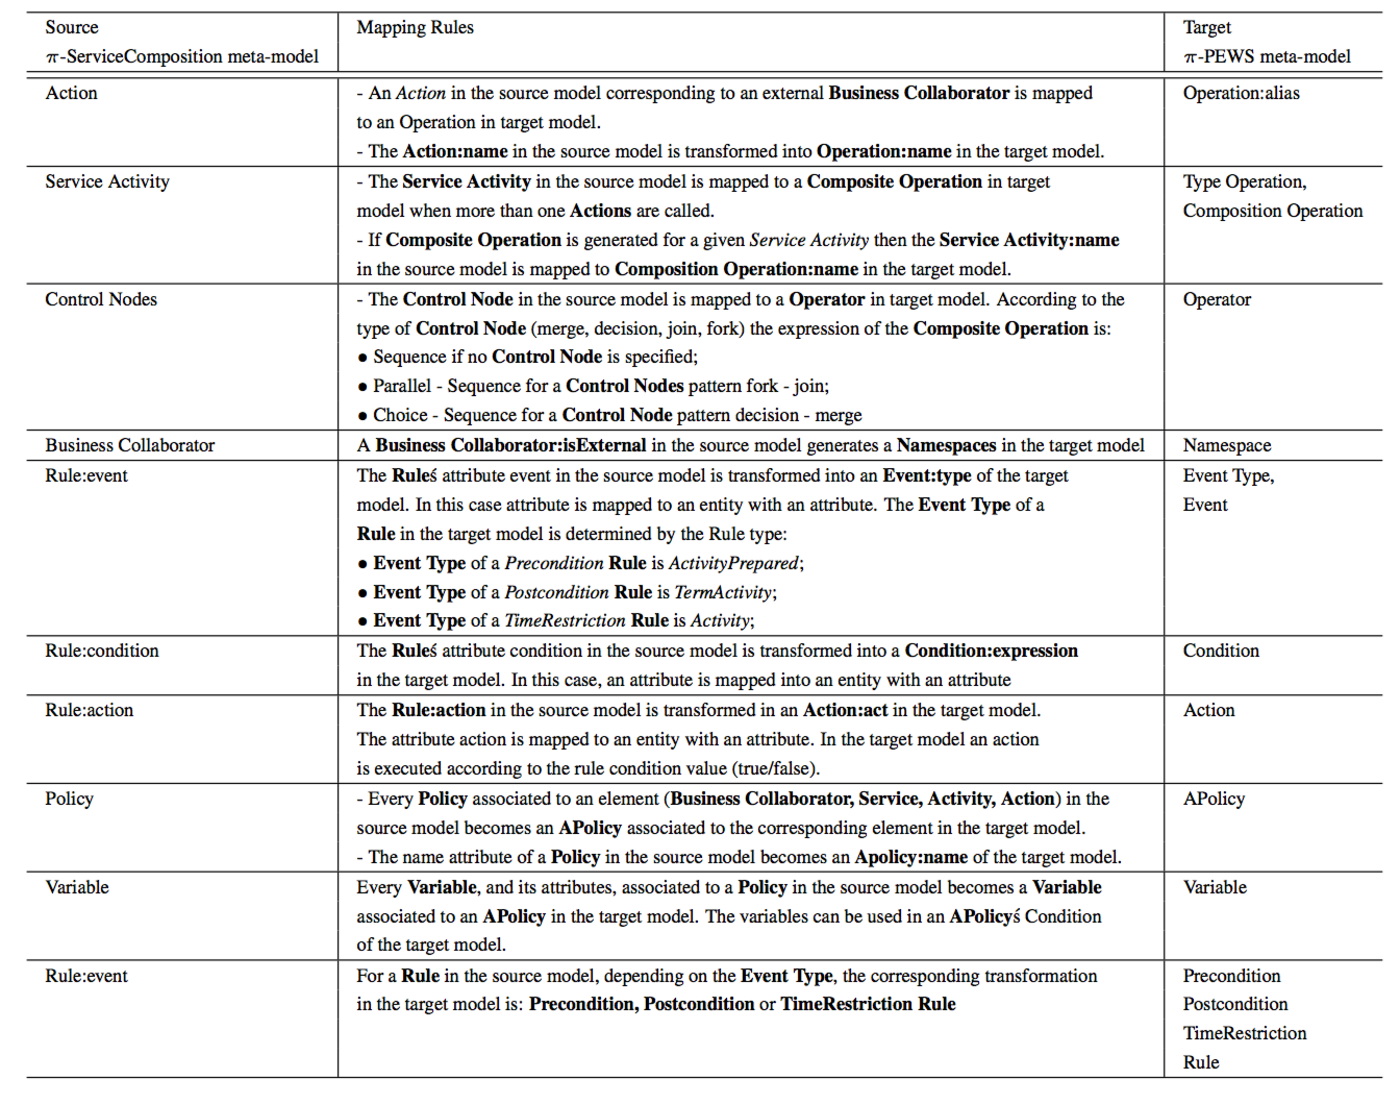
\includegraphics[width=0.96\textwidth]{figs/Table7}}
%\caption{Transformation Rules: From $\pi$-ServiceComposition to $\pi$-PEWS}
%\label{fig:ServiceComposition-Pews-Rules}
%\end{figure}


The A-policies defined for the entities of a $\pi$-service composition model are transformed into {\sf A-policy} entities, named according to the names expressed in the source model. The transformation of the rules expressed in a $\pi$-service composition is guided by the event types associated to these rules. The variables associated to an A-policy expressed in a $\pi$-service composition model as {\sf $<$Variable:name, Variable:type$>$} are transformed into entities  {\sf Variable} with attributes {\sf Name} and {\sf Type} directly specified from the elements {\sf Variable:name} and {\sf Variable:type} of a $\pi$-service composition model.

%As shown in Table \ref{fig:ServiceComposition-Pews-Rules}, 
For an event of type Pre the corresponding transformed rule is a {\sf Precondition}; for an event of type Post the corresponding transformed rule is a {\sf Post- condition}; finally, for an event of type TimeRestriction the corresponding transformed rule is a {\sf Time}. The condition expression of a rule in a $\pi$-service composition ({\sf Rule:condition}) is transformed into a  {\sf Condition:expression} where the attributes of the expression are transformed into  entities {\sf Attribute}.

Figure \ref{fig:Specific-Contract-Representation} shows the $\pi$-PEWS code resulting from the $\pi$- service composition model  of our scenario example.

\begin{figure}
\centering{
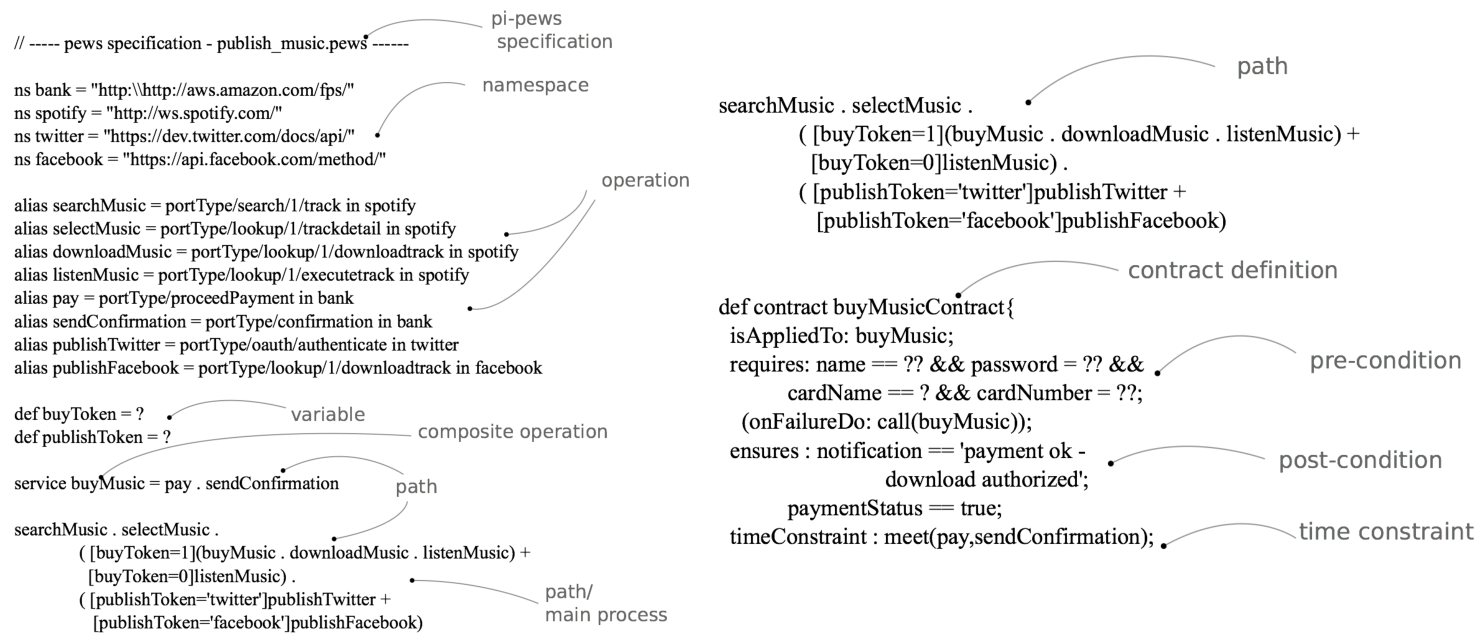
\includegraphics[width=0.96\textwidth]{figs/31-31}}
\caption{$\pi$-PEWS Specific and Contract Representation}
\label{fig:Specific-Contract-Representation}
\end{figure}

\subsection{Implementation}
We have provided tools for aiding the user into transform models for all the levels, except for the CIM into PIM level, which should be manually performed.




This section  describes the $\pi$-SOD-M development environment that implements the generation of {\em A-policies}' based services' compositions. For a given services' based application, the process  consists in generating the  code starting from a $\pi$-SCM modeling an application. Note that the services' composition model is not modeled from scratch, but it is the result of a general process defined by the $\pi$-SOD-M method in which a set of models are built following a service oriented approach \cite{decastro1}.

%We used the Eclipse Modeling Framework (EMF) to implement the whole model transformation process \footnote {The EMF project is a modeling framework and code generation facility for building tools and other applications based on a structured data model.}. From a model specification described in XMI, EMF provides tools and runtime support to produce a set of Java classes for the model, along with a set of adapter classes that enable viewing and command-based editing of the model, and a basic editor.
%In order to automate the transformation we specified  transformation rules using the ATL model transformation language Finally, in order to generate code we  used Acceleo \footnote{http://www.acceleo.org/pages/home/en}.

%%..--..--..--..--..--..--..--..--..--..--..--..--..--..--..--..--..--..--..--..--..--..--..--..--..--..--..--..--..--..--..--..--..--..--..--..--..--..--
\subsection{General architecture}
%%..--..--..--..--..--..--..--..--..--..--..--..--..--..--..--..--..--..--..--..--..--..--..--..--..--..--..--..--..--..--..--..--..--..--..--..--..--..--

Figure \ref{fig:policymanager} depicts a general architecture of the $\pi$-SOD-M Development Environment showing the set of plug-ins  developed in order to implement it. The environment implements the abstract architecture. Thus, it consists of plug-ins implementing the $\pi$-SCM and $\pi$-{\sc Pews} meta-models used for defining models specifying services' compositions and their associated policies; and ATL rules for transforming  PSM models (model to model transformation) and finally generating code (model to text transformation).
\begin{figure}[t]
	\begin{center}
		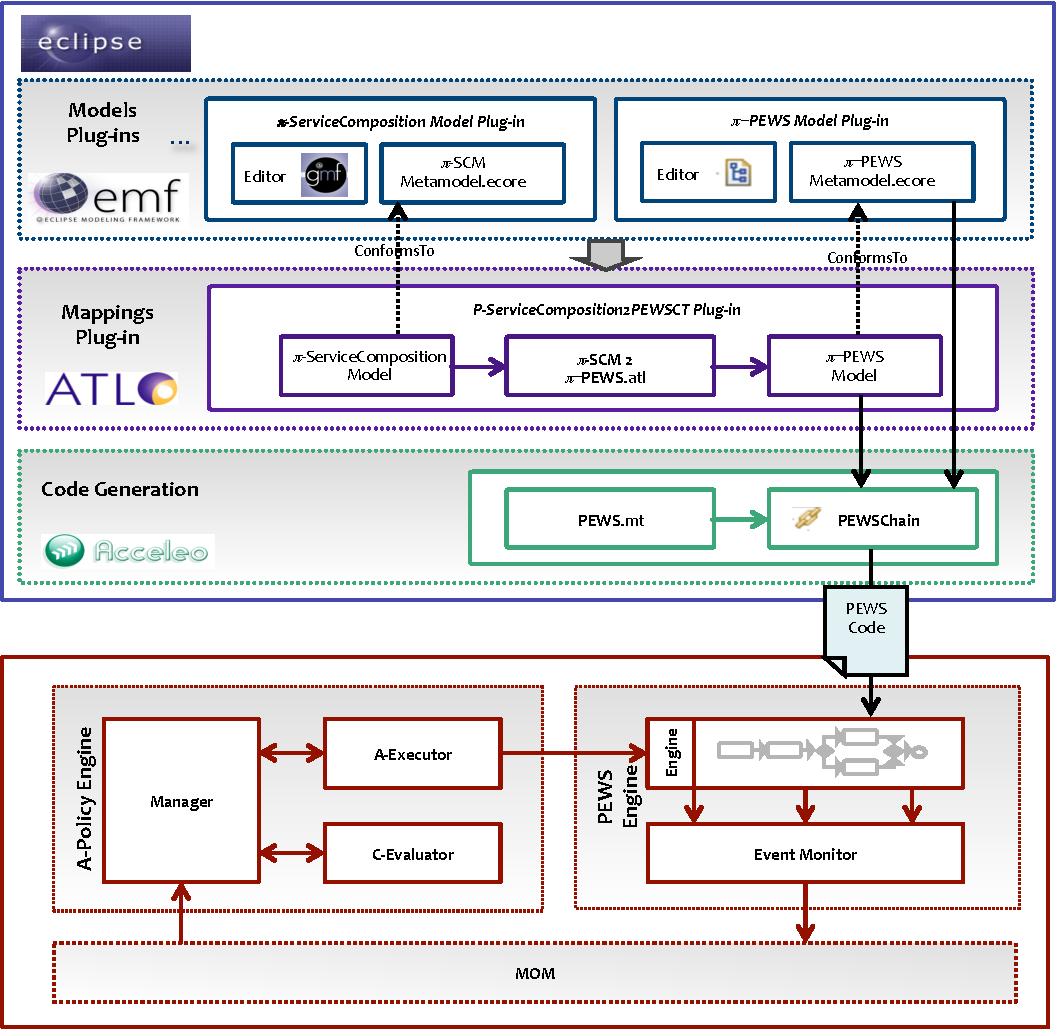
\includegraphics[width=0.60\textwidth]{figs/architecture}
	\end{center}
		\caption{$\pi$-SOD-M Development Environment}
   \label{fig:policymanager}
\end{figure}
\begin{itemize}
\item 	We  used the Eclipse Modeling Framework (EMF) \footnote {The EMF project is a modeling framework and code generation facility for building tools and other applications based on a structured data model.}   for implementing the meta-models  $\pi$- SCM and $\pi$-{\sc Pews}. Then, starting form these meta-models, we  developed the models' plug-ins needed to support the graphical representation of the $\pi$- SCM and $\pi$-{\sc Pews} models ($\pi$-ServiceCompostion Model and $\pi$-PEWS Model plug-ins).

\item	 We used  ATL \footnote{http://eclipse.org/atl/. An ATL program is basically a set of rules that define how source model elements are matched and navigated to create and initialize the elements of the target models.}
for  developing the mapping plug-in implementing the  mappings between models ($\pi$-ServiceComposition2$\pi$-PEWS Plug-in).

\item 	We  used Acceleo \footnote{http://www.acceleo.org/pages/home/en} for implementing  the code generation plug-in. We coded the pews.mt program  that implements the model to text transformation for generating executable code. It takes as input a $\pi$-PEWS model implementing a specific services' composition and it generates the code to be executed by the 
{\em A-policy} based services' composition execution environment. 

%\item Finally, we created a chain execution  to execute the model to text transformation.
\end{itemize}


%%..--..--..--..--..--..--..--..--..--..--..--..--..--..--..--..--..--..--..--..--..--..--..--..--..--..--..--..--..--..--..--..--..--..--..--..--..--..--
\subsection{A-policy manager}
%..--..--..--..--..--..--..--..--..--..--..--..--..--..--..--..--..--..--..--..--..--..--..--..--..--..--..--..--..--..--..--..--..--..--..--..--..--..--

As  shown in Figure \ref{fig:policymanager}, once an instance of a PEWS code is obtained starting form a particular $\pi$-services' composition model it can be executed over {\em A-policy} based services' composition execution environment  consisting of a composition engine and a {\em A-policy} manager.  The  {\em A-policy} manager  consists of three main components Manager, for scheduling the execution of rules, C-Evaluator and A-Executor respectively for evaluating rules' conditions and executing their actions. The {\em A-policy} Manager interacts with a composition engine thanks to a  message communication layer (MOM).


The composition engine manages the life cycle of the composition. Once a composition instance is activated, the engine schedules the composition activities according to the composition control flow.
Each activity is seen as the process where the service method call is executed.
The execution of an activity has four states: prepared, started, terminated, and failure.
The execution of the control flow (sequence, and/or split and join) can also be prepared, started, terminated and raise a failure.

At execution time, the evaluation of policies done by the {\em A-policy} manager must be synchronized with the execution of the services' composition (i.e., the execution of an activity or a control flow).  Policies associated to a scope are activated when the execution of its scope starts. A {\em A-policy} will have to be executed only if one or several of its rules is triggered. If several rules are triggered the {\em A-policy} manager first builds an execution plan that specifies the order in which such rules will be executed according to the strategies defined in the following section. 
%Once rules have been executed, the {\em A-policy} finishes its execution and returns to a sleeping state.
If rules belonging to several policies are triggered then policies are also ordered according to an execution plan. The execution of policies is out of the scope of this paper, the interested reader can refer to \cite{Espinosa-Oviedo2011a} for further details.
%The order of policies has implications on the global order of the rules to be executed.


